\documentclass[aspectratio=169]{beamer}

\usetheme{Madrid}
\usecolortheme{seahorse}
\usepackage[utf8]{inputenc}
\usepackage{amsmath}
\usepackage{listings}
\usepackage{xcolor}
\usepackage{graphicx}
\usepackage{booktabs}

\lstdefinestyle{cli}{
  basicstyle=\ttfamily\scriptsize,
  backgroundcolor=\color{black!5},
  frame=single,
  breaklines=true,
  columns=fullflexible,
  keywordstyle=\color{blue},
}
\lstdefinestyle{va}{
  basicstyle=\ttfamily\scriptsize,
  backgroundcolor=\color{black!5},
  frame=single,
  breaklines=true,
  columns=fullflexible,
}
\lstnewenvironment{cli}{\lstset{style=cli}}{}
\lstnewenvironment{va}{\lstset{style=va}}{}

\title{Building openMemristorPDK, From Scratch}
\subtitle{A bare-minimum, multi-material memristor PDK -- layers through simulation, entirely through openPDKcreator's own GUI}
\author{}
\date{}

\begin{document}

\frame{\titlepage}

% ---------------------------------------------------------------
\begin{frame}{Goal}
\begin{itemize}
  \item A genuinely \textbf{minimum} PDK for a two-terminal memristor device
        family, built entirely through \texttt{openPDKcreator}'s own real
        GUI/launcher -- the same tool hardened over many sessions against
        IHP's real SG13G2 PDK.
  \item \textbf{Two switching-oxide materials} (TiO$_2$, HfO$_2$) and
        \textbf{three top-electrode metals} (Au, Ti, Al) -- bottom
        electrode always Au -- giving three real device variants.
  \item \textbf{Two genuinely different} Verilog-A compact models: one
        shared by both TiO$_2$ variants (same equations, different
        parameter sets), a structurally different one for HfO$_2$.
  \item Real process corners, a real xschem symbol + schematic, and a
        real \texttt{ngspice}/OSDI simulation for every variant.
  \item This deck assumes nothing from any earlier session -- every
        step, from an empty directory to real simulated waveforms, is
        shown here.
\end{itemize}
\end{frame}

% ---------------------------------------------------------------
\begin{frame}{The three real device variants}
\begin{center}
\begin{tabular}{lccl}
\toprule
Cell & Bottom electrode & Oxide & Top electrode \\
\midrule
\texttt{memristor\_tio2\_au} & Au & TiO$_2$ & Au \\
\texttt{memristor\_tio2\_ti} & Au & TiO$_2$ & Ti \\
\texttt{memristor\_hfo2\_al} & Au & HfO$_2$ & Al \\
\bottomrule
\end{tabular}
\end{center}
\vspace{0.5em}
Plus the original, generic \texttt{memristor} cell (Au/TiO$_2$/Au, the
same composition as the first variant) from this project's own very
first build session -- kept, and given real port geometry alongside
the three new variants, rather than discarded.
\end{frame}

% ---------------------------------------------------------------
\begin{frame}[fragile]{Independent project, real launcher}
Reachable inside the running IIC-OSIC-TOOLS container -- own
directory, own git history, nothing shared with the IHP-based
project:
\begin{cli}
cd /foss/designs/openMemristorPDK
python3 main.py --pdk-root data/openmemristorpdk gui
\end{cli}
Every real step in this deck -- layers, Magic Tech, DRC, LEF macros
and their own port geometry, Library Manager, xschem symbol/schematic
-- was driven through this exact real launcher, the actual running
Tk GUI (captured live via VNC), not a headless script standing in
for it.
\end{frame}

% ---------------------------------------------------------------
\begin{frame}{The PDK Wizard's own Analog/Memristor path}
\begin{center}
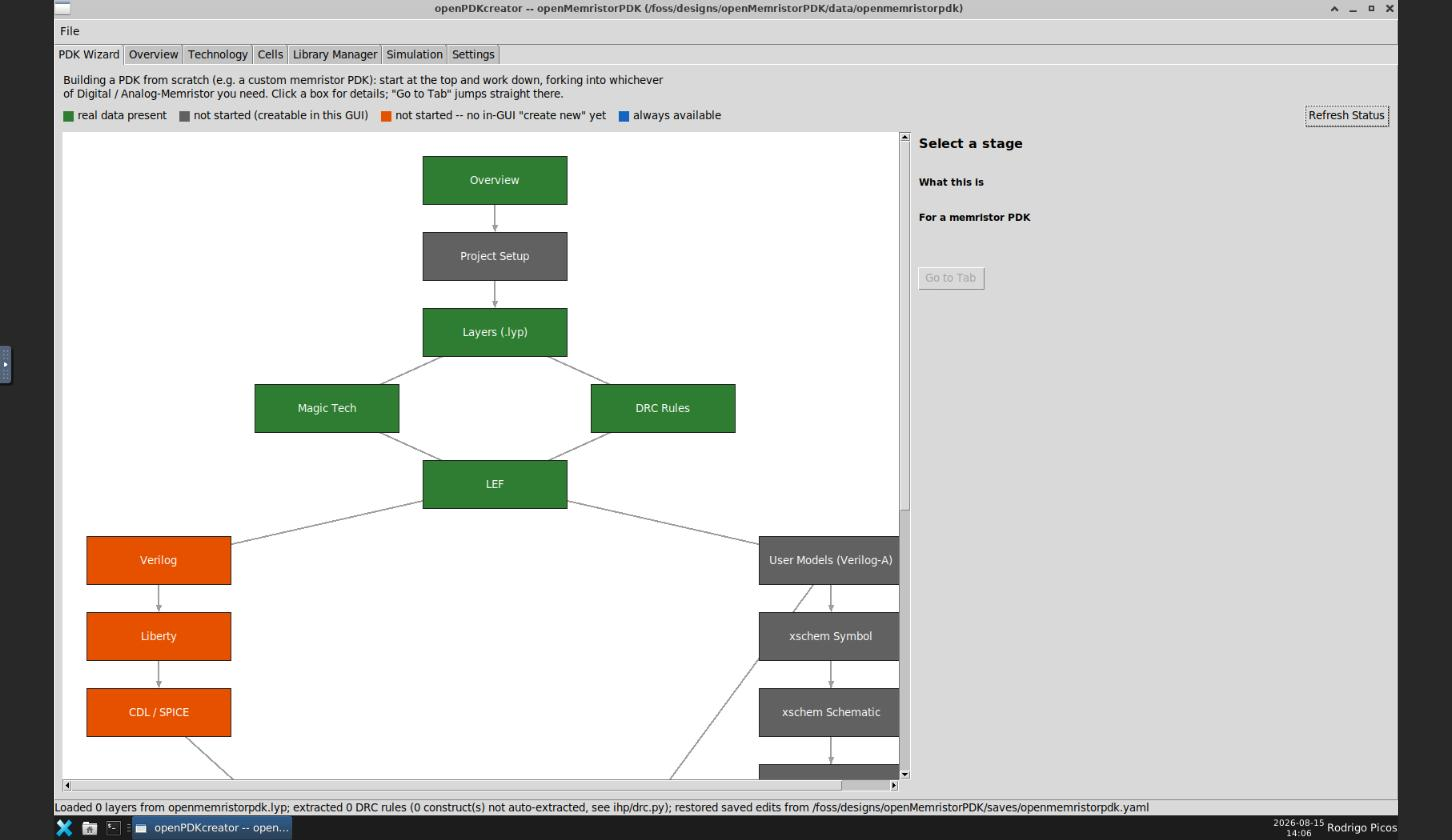
\includegraphics[width=0.72\textwidth]{figures/pdk_wizard.jpg}
\end{center}
\footnotesize
Green = real data present. The wizard forks Digital vs.
Analog/Memristor -- this build follows the right-hand fork: Layers
$\to$ Magic Tech / DRC $\to$ LEF $\to$ User Models (Verilog-A) $\to$
xschem Symbol/Schematic. (Captured during this project's first build
session -- the wizard's own layout is unchanged, only the underlying
project data has grown considerably since.)
\end{frame}

% ---------------------------------------------------------------
\begin{frame}{Layers: a 6-layer, 2-material stack}
Technology $\to$ Layers $\to$ \textbf{New .lyp File...}, then
\textbf{New Layer} $\times 6$:
\begin{center}
\begin{tabular}{lccl}
\toprule
Name & GDS layer/dt & Purpose & Role \\
\midrule
BE\_Au.drawing & 10/0 & drawing & Bottom electrode (Au, always) \\
MEM\_TiO2.drawing & 11/0 & drawing & TiO$_2$ switching oxide \\
MEM\_HfO2.drawing & 12/0 & drawing & HfO$_2$ switching oxide \\
TE\_Au.drawing & 20/0 & drawing & Top electrode (Au) \\
TE\_Ti.drawing & 21/0 & drawing & Top electrode (Ti) \\
TE\_Al.drawing & 22/0 & drawing & Top electrode (Al) \\
\bottomrule
\end{tabular}
\end{center}
\vspace{0.3em}
\footnotesize
Fictional, illustrative GDS numbers/colors -- a demo stack, not a
qualified process. Exported via File $\to$ \textbf{Export Edited
Layers} to \texttt{export/openmemristorpdk/libs.tech/klayout/tech/*.lyp},
a real, valid, open\_pdks-format KLayout layer file.
\end{frame}

% ---------------------------------------------------------------
\begin{frame}{Magic Tech + DRC Rules}
\begin{columns}
\column{0.5\textwidth}
\textbf{Magic Tech} (Technology $\to$ Magic Tech):
\begin{itemize}
  \item \textbf{New .tech File...}
  \item 2 real planes: \texttt{metal}, \texttt{oxide}
  \item 6 real types, one per layer above (\texttt{be\_au},
        \texttt{te\_au}, \texttt{te\_ti}, \texttt{te\_al} on
        \texttt{metal}; \texttt{mem\_tio2}, \texttt{mem\_hfo2} on
        \texttt{oxide})
\end{itemize}
\column{0.5\textwidth}
\textbf{DRC Rules} (Technology $\to$ DRC Rules), 4 real rules:
\begin{itemize}
  \item \texttt{BE.W.1}: min.\ width, Au BE, 0.2\,\textmu m
  \item \texttt{MEM1.W.1}: min.\ width, TiO$_2$, 0.1\,\textmu m
  \item \texttt{MEM2.W.1}: min.\ width, HfO$_2$, 0.1\,\textmu m
  \item \texttt{TE.S.1}: min.\ spacing, Au TE, 0.15\,\textmu m
\end{itemize}
\end{columns}
\vspace{0.5em}
Both exported via File $\to$ \textbf{Save Edits} / Export $\to$
\textbf{Export Edited Magic Types} / \textbf{Export Edited DRC Rules}
-- real, generated KLayout DRC Ruby (\texttt{custom\_rules.drc}) for
every rule, since none of these came from a real, downloaded deck to
patch instead.
\end{frame}

% ---------------------------------------------------------------
\begin{frame}[fragile]{LEF: 4 real macros, real port geometry}
Cells $\to$ LEF $\to$ type a path $\to$ \textbf{Create File}, then --
unlike this project's own first build session -- a real \textbf{New
Macro...} action now exists in the GUI (added during this same
overall effort): \texttt{memristor\_tio2\_au}, \texttt{memristor\_tio2\_ti},
\texttt{memristor\_hfo2\_al}, each \texttt{CLASS CORE}, \texttt{SIZE
1.0 BY 1.0}, \texttt{SITE CoreSite}, with real \texttt{BE}/\texttt{TE}
pins (\texttt{New Pin}, both \texttt{INOUT}/\texttt{SIGNAL}).
\medskip

Each pin's own real \texttt{PORT} geometry was drawn through a new
\textbf{Edit Geometry...} dialog (a real, interactive canvas, the
same shared widget xschem/Qucs-S symbol editing already used) -- BE
on \texttt{BE\_Au.drawing}, TE on the matching real top-electrode
layer for that variant:
\begin{va}
PIN BE
  PORT LAYER BE_Au.drawing ; RECT 0 0 1 1 ; END
END BE
PIN TE
  PORT LAYER TE_Ti.drawing ; RECT 0 0 1 1 ; END
END TE
\end{va}
File $\to$ \textbf{Save Edits} persists all 4 macros (a real,
found-and-fixed bug meant a brand-new macro used to vanish on
reload -- see the next slide).
\end{frame}

% ---------------------------------------------------------------
\begin{frame}{A real, found bug: new macros didn't survive reload}
\begin{itemize}
  \item Building this PDK's own 3 new LEF macros surfaced a real,
        pre-existing gap in \texttt{openPDKcreator} itself: a
        brand-new macro's \emph{pins} were saved by name, but the
        macro's own identity (class/size/site/origin) was not --
        the only thing that makes that name resolvable again.
  \item A fresh reload re-parsed the real, unmodified source file,
        found no macro by that name, and silently dropped the
        orphaned pin data too. 3 of this project's own 4 macros were
        lost this way before the bug was found.
  \item Fixed upstream in \texttt{openPDKcreator} itself (a new
        \texttt{lef\_macros} save key, reconstructed on load before
        pins are re-attached) -- verified against a fresh, separate
        \texttt{App} instance, then used to rebuild this project's
        own 4 macros properly, this time surviving a real save +
        reload.
\end{itemize}
\end{frame}

% ---------------------------------------------------------------
\begin{frame}{Library Manager: the real payoff}
\begin{center}
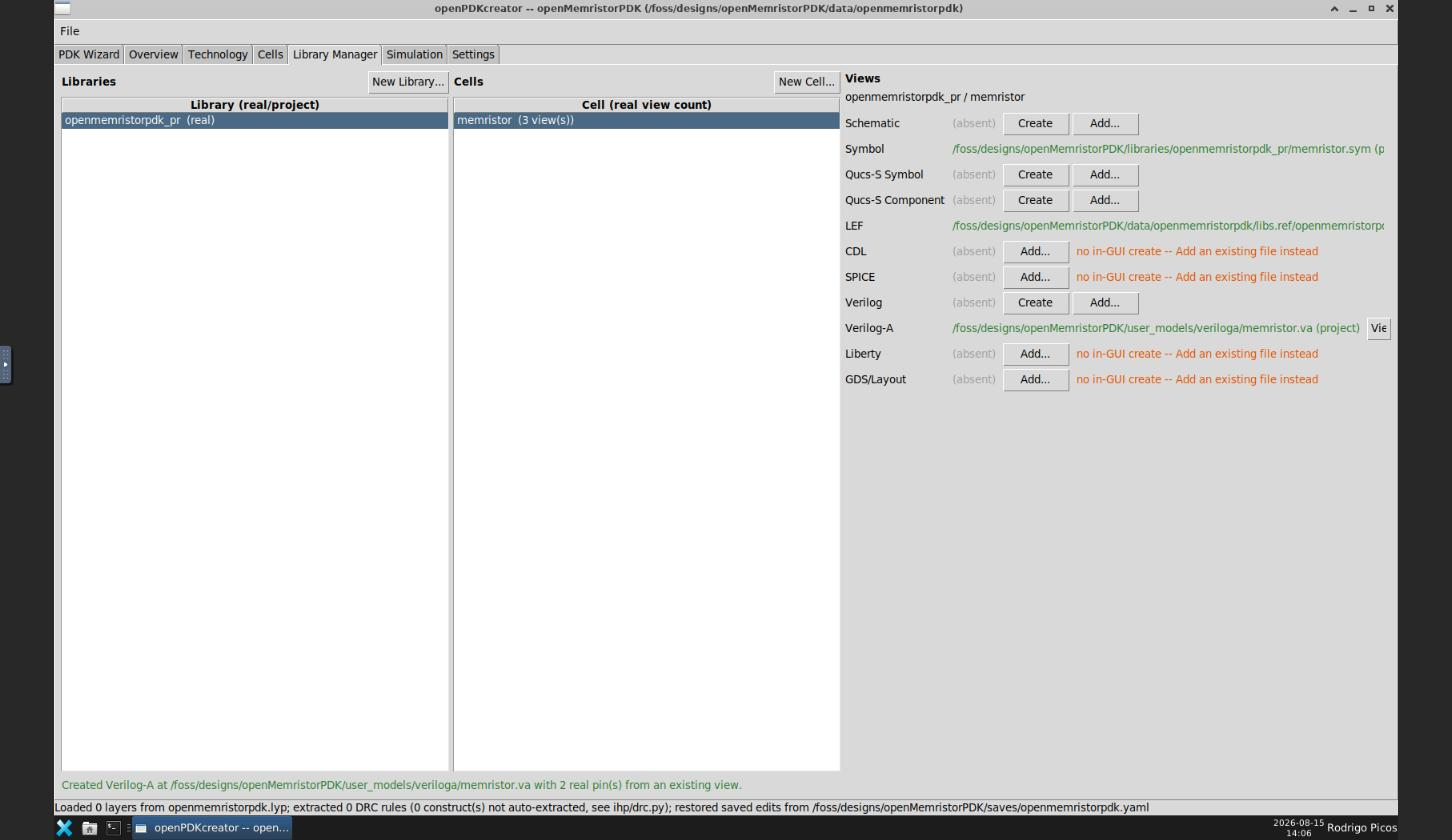
\includegraphics[width=0.95\textwidth]{figures/library_manager.jpg}
\end{center}
\footnotesize
Auto-discovers every real LEF macro as a library/cell (here,
\texttt{openmemristorpdk\_pr} / \texttt{memristor}), and is the real
hub for creating/linking every other view (Verilog-A, xschem
symbol/schematic) against that same cell name.
\end{frame}

% ---------------------------------------------------------------
\begin{frame}{Two genuinely different Verilog-A models}
Per the task's own real requirement: a \emph{model}, not just a
parameter set, must differ between the two switching-oxide materials.
\begin{columns}
\column{0.55\textwidth}
\textbf{Model 1 -- linear ion drift}\\
\footnotesize
\texttt{memristor\_tio2\_au.va} / \texttt{memristor\_tio2\_ti.va}:
identical equations, different default \texttt{Ron}/\texttt{Roff}/
\texttt{uv} (Ti's own more resistive top contact vs.\ Au's).
Strukov, Snider, Stewart \& Williams, \emph{``The missing memristor
found''}, Nature 453, 80--83 (2008).
\column{0.45\textwidth}
\textbf{Model 2 -- bipolar threshold switching}\\
\footnotesize
\texttt{memristor\_hfo2\_al.va}: a structurally different,
filamentary-conduction model -- the real, standard picture for
HfO$_2$ RRAM, not boundary drift. In the general lineage of Kvatinsky
et al., ``TEAM: ThrEshold Adaptive Memristor Model'', IEEE TCAS-I
60(1) (2013).
\end{columns}
\end{frame}

% ---------------------------------------------------------------
\begin{frame}{Model 1: linear ion-drift equations}
A thin oxide film of thickness $D$ between two electrodes (BE, TE);
one region doped (low resistance $R_{on}$), the other undoped
($R_{off}$). State $x = w/D \in [0,1]$: the doped/undoped boundary
position.
\[
\frac{dx}{dt} = \frac{\mu_v R_{on}}{D^2}\, i(t)
\qquad
R_{mem}(x) = R_{on}\,x + R_{off}\,(1-x)
\qquad
v = R_{mem}(x)\, i
\]
\vspace{0.3em}
\begin{center}
\begin{tabular}{lccc}
\toprule
Variant & $R_{on}$ & $R_{off}$ & $\mu_v$ \\
\midrule
Au top (\texttt{memristor\_tio2\_au}) & 100\,$\Omega$ & 16\,k$\Omega$ & $1\times10^{-14}$ \\
Ti top (\texttt{memristor\_tio2\_ti}) & 250\,$\Omega$ & 20\,k$\Omega$ & $0.8\times10^{-14}$ \\
\bottomrule
\end{tabular}
\end{center}
\footnotesize
Illustrative, not measured -- there is no real fabricated silicon
behind this from-scratch teaching PDK to calibrate against; only the
\emph{direction} (Ti's more resistive contact) is real physics.
\end{frame}

% ---------------------------------------------------------------
\begin{frame}{Model 2: bipolar threshold switching}
A real state variable that only moves once the real terminal voltage
crosses a real threshold (SET/RESET), with an exponential
(tunneling-like) state-to-resistance mapping instead of a linear one
-- the real, qualitative signature of filamentary conduction.
\[
\frac{dx}{dt} =
\begin{cases}
(v - V_{on})/\tau & v > V_{on} \\
(v - V_{off})/\tau & v < V_{off} \\
0 & \text{otherwise}
\end{cases}
\qquad
R_{mem}(x) = R_{off}\, e^{-x \ln(R_{off}/R_{on})}
\]
\vspace{0.3em}
\begin{center}
\begin{tabular}{cccc}
\toprule
$R_{on}$ & $R_{off}$ & $V_{on}$ & $V_{off}$ \\
\midrule
500\,$\Omega$ & 50\,k$\Omega$ & 0.8\,V & $-$0.6\,V \\
\bottomrule
\end{tabular}
\end{center}
\end{frame}

% ---------------------------------------------------------------
\begin{frame}[fragile]{Compiling and instantiating -- real gotchas}
\begin{cli}
openvaf memristor_tio2_au.va --output memristor_tio2_au.osdi
openvaf memristor_tio2_ti.va --output memristor_tio2_ti.osdi
openvaf memristor_hfo2_al.va --output memristor_hfo2_al.osdi
\end{cli}
All three compile clean. Real, empirically-confirmed conventions
(carried over from this project's own first device, still true
here):
\begin{itemize}
  \item \texttt{osdi <file>.osdi} must be pre-loaded via a
        \texttt{.spiceinit} in the working directory, \emph{before}
        any \texttt{.model} card referencing it is parsed.
  \item OSDI compact models instantiate with an \texttt{n} prefix
        (\texttt{n1 be te modelname}), not a SPICE built-in letter.
  \item Model parameters belong on the \texttt{.model} card, not the
        instance line.
\end{itemize}
\end{frame}

% ---------------------------------------------------------------
\begin{frame}[fragile]{Real transient testbenches, one per variant}
\begin{va}
.model mm memristor_tio2_au ron=100 roff=16k d=10n uv=1e-14 x0=0.3
n1 te 0 mm
vte te 0 dc 0 sin(0 1.0 0.6)
.tran 300u 3.34
\end{va}
Same real shape for all three variants (\texttt{docs/simulation/
memristor\_tio2\_au/}, \texttt{.../memristor\_tio2\_ti/},
\texttt{.../memristor\_hfo2\_al/}), each with its own real
\texttt{run\_simulation.sh}:
\begin{cli}
openvaf <variant>.va --output <variant>.osdi
ngspice -b mem_tran.sp
python3 plot_memristor.py
\end{cli}
The HfO$_2$/Al variant uses a larger drive (1.2\,V, 25\,Hz) and an
overridden \texttt{tau} to make its own real, fast threshold-switching
dynamics visible at a demo-friendly timescale.
\end{frame}

% ---------------------------------------------------------------
\begin{frame}{Result: Au/TiO$_2$/Au -- classic pinched hysteresis}
\begin{center}
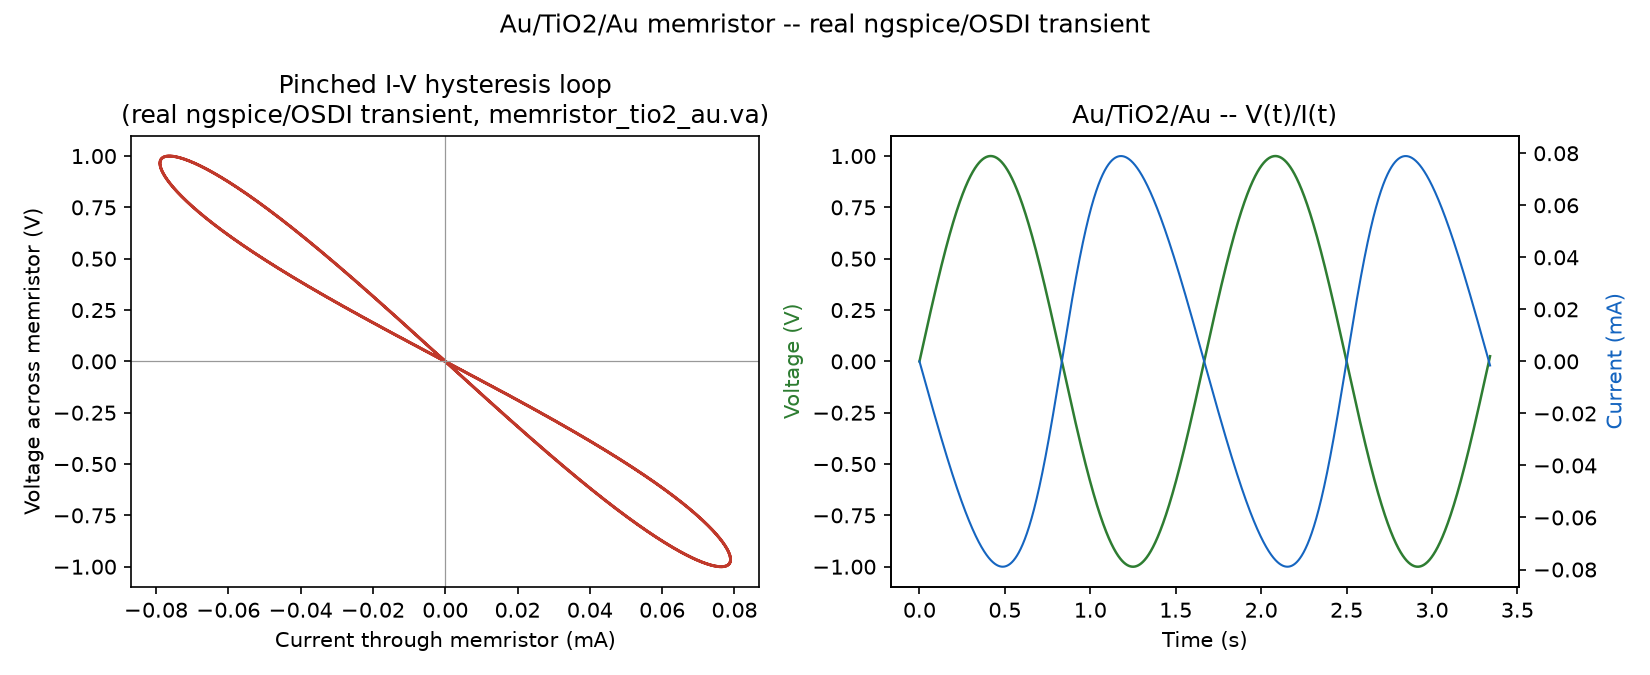
\includegraphics[width=0.85\textwidth]{figures/memristor_tio2_au_transient.png}
\end{center}
\footnotesize
Real, simulated data -- the I-V loop pinches exactly at the origin
every half-cycle, the defining memristor fingerprint.
\end{frame}

% ---------------------------------------------------------------
\begin{frame}{Result: Au/TiO$_2$/Ti -- same model, shifted window}
\begin{center}
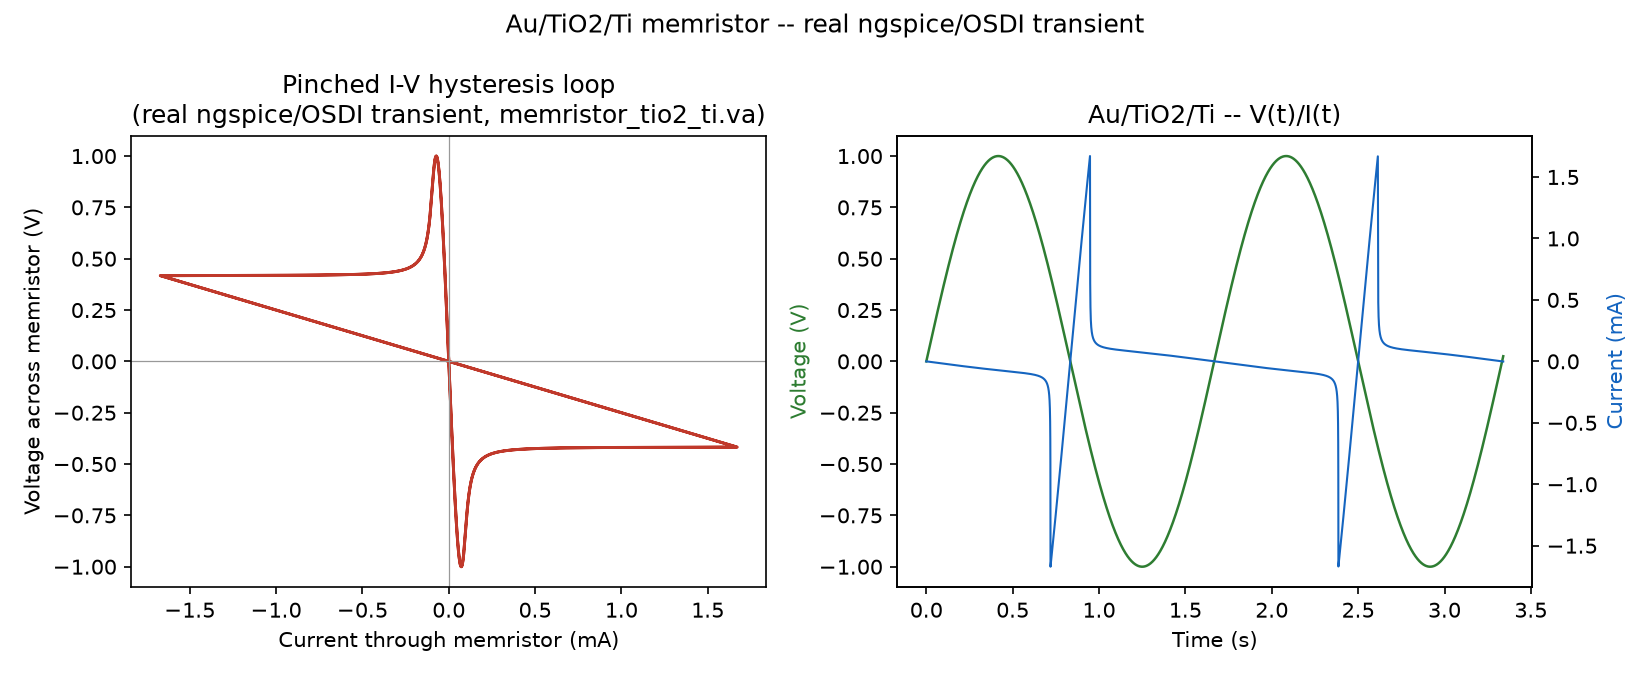
\includegraphics[width=0.85\textwidth]{figures/memristor_tio2_ti_transient.png}
\end{center}
\footnotesize
Same real linear ion-drift model, same real drive -- a visibly
different loop shape purely from Ti's own higher $R_{on}$/lower
$\mu_v$ parameter set (this real trajectory happens to reach full
saturation, $R \in [250, 20\,\mathrm{k}]\,\Omega$ exactly, unlike the
Au-top variant).
\end{frame}

% ---------------------------------------------------------------
\begin{frame}{Result: Au/HfO$_2$/Al -- a genuinely different signature}
\begin{center}
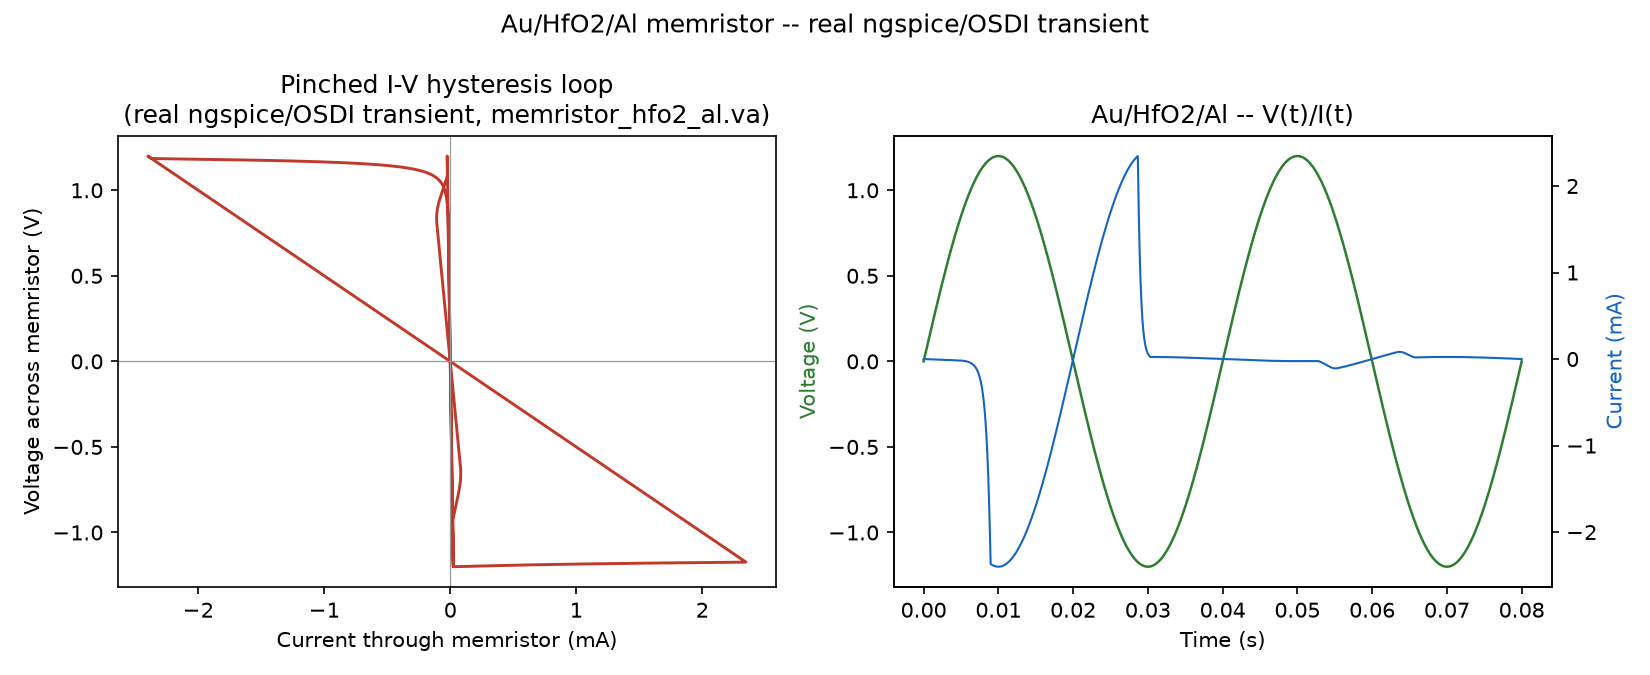
\includegraphics[width=0.85\textwidth]{figures/memristor_hfo2_al_transient.png}
\end{center}
\footnotesize
Sharp SET/RESET current spikes at the real threshold voltages, flat
elsewhere -- qualitatively different from the smooth TiO$_2$ loops
above, real, direct confirmation that this is a genuinely different
model, not a relabeled copy.
\end{frame}

% ---------------------------------------------------------------
\begin{frame}[fragile]{Real process corners}
The Simulation tab's own Corners sub-tab (real ngspice
\texttt{.LIB...ENDL} PVT-corner blocks) was, until this same overall
effort, deliberately \textbf{read-only}. Made genuinely editable --
New/Delete Corner, a per-corner \texttt{key = value} param form --
and used here to author real corners for all three variants:
\begin{va}
.LIB TT
.param ron_tio2_au = 100
.param roff_tio2_au = 16k
... (ron/roff for all 3 variants) ...
.ENDL TT

.LIB FF   /* -20% on every real Ron/Roff */
.LIB SS   /* +20% */
\end{va}
\texttt{data/openmemristorpdk/libs.tech/ngspice/models/
openmemristorpdk\_corners.lib}, created via the GUI's own
\textbf{Create File} action, edited through the new real form.
\end{frame}

% ---------------------------------------------------------------
\begin{frame}{Result: a real TT/FF/SS corner sweep}
\begin{center}
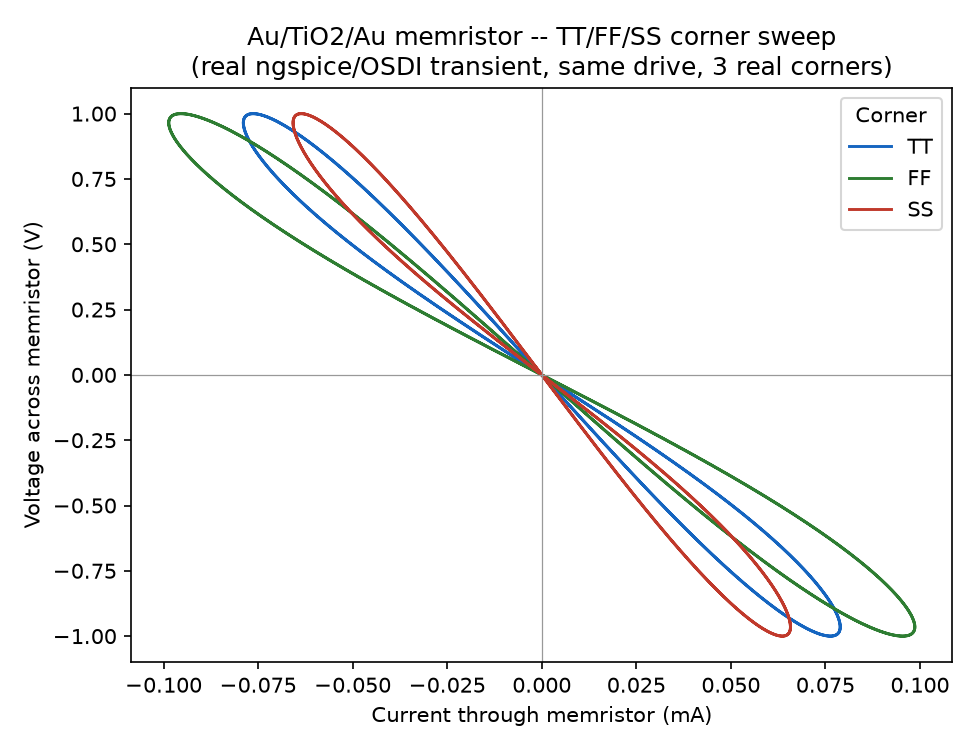
\includegraphics[width=0.78\textwidth]{figures/memristor_corners_transient.png}
\end{center}
\footnotesize
Au/TiO$_2$/Au, same real drive, three real corner runs via
\texttt{.lib openmemristorpdk\_corners.lib \{TT,FF,SS\}} +
\texttt{\{ron\_tio2\_au\}}-style parameter overrides on the
\texttt{.model} line -- FF shows the widest current swing (lowest
resistance window), SS the narrowest, exactly as the real $\pm$20\%
spread intends.
\end{frame}

% ---------------------------------------------------------------
\begin{frame}{A real xschem symbol -- via the real GUI, and launcher}
\begin{center}
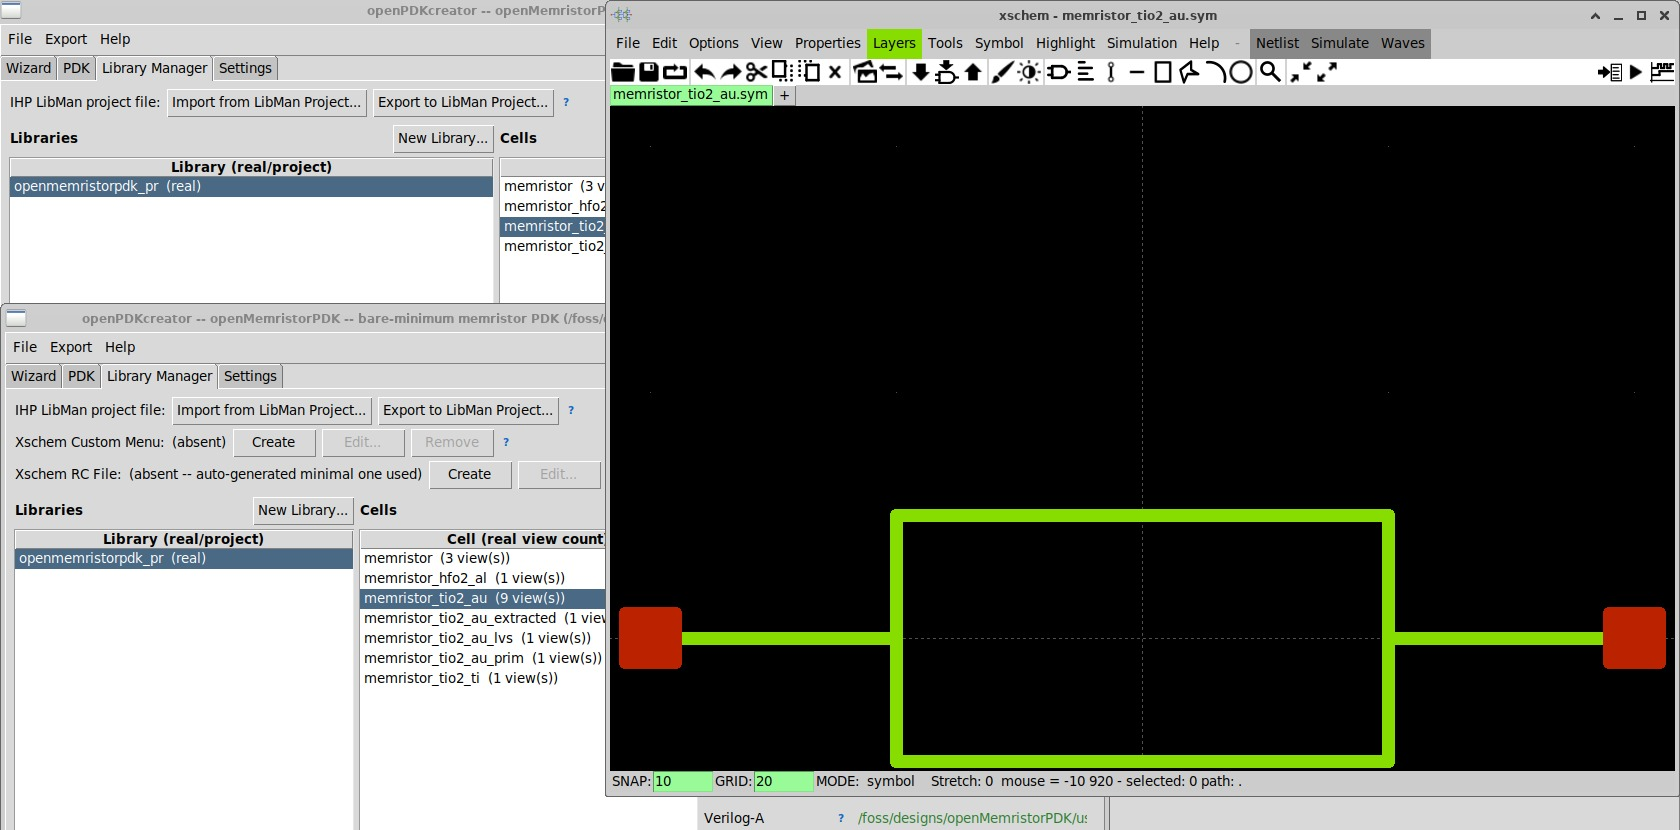
\includegraphics[width=0.55\textwidth]{figures/xschem_memristor_symbol.jpg}
\end{center}
\footnotesize
Cells $\to$ xschem $\to$ Symbols $\to$ \textbf{Create File}, real
\textbf{New Port} $\times$2 (BE, TE, both \texttt{inout}), then a
real box body drawn with the Graphical sub-tab's own Line tool --
confirmed by actually launching real xschem on the exported file the
same way \texttt{gui/library\_manager\_view.py}'s own \textbf{Open in
xschem} action would (\texttt{xschem <path>}, from the project root).
\end{frame}

% ---------------------------------------------------------------
\begin{frame}{A real xschem schematic -- and a real netlisting gotcha}
\begin{center}
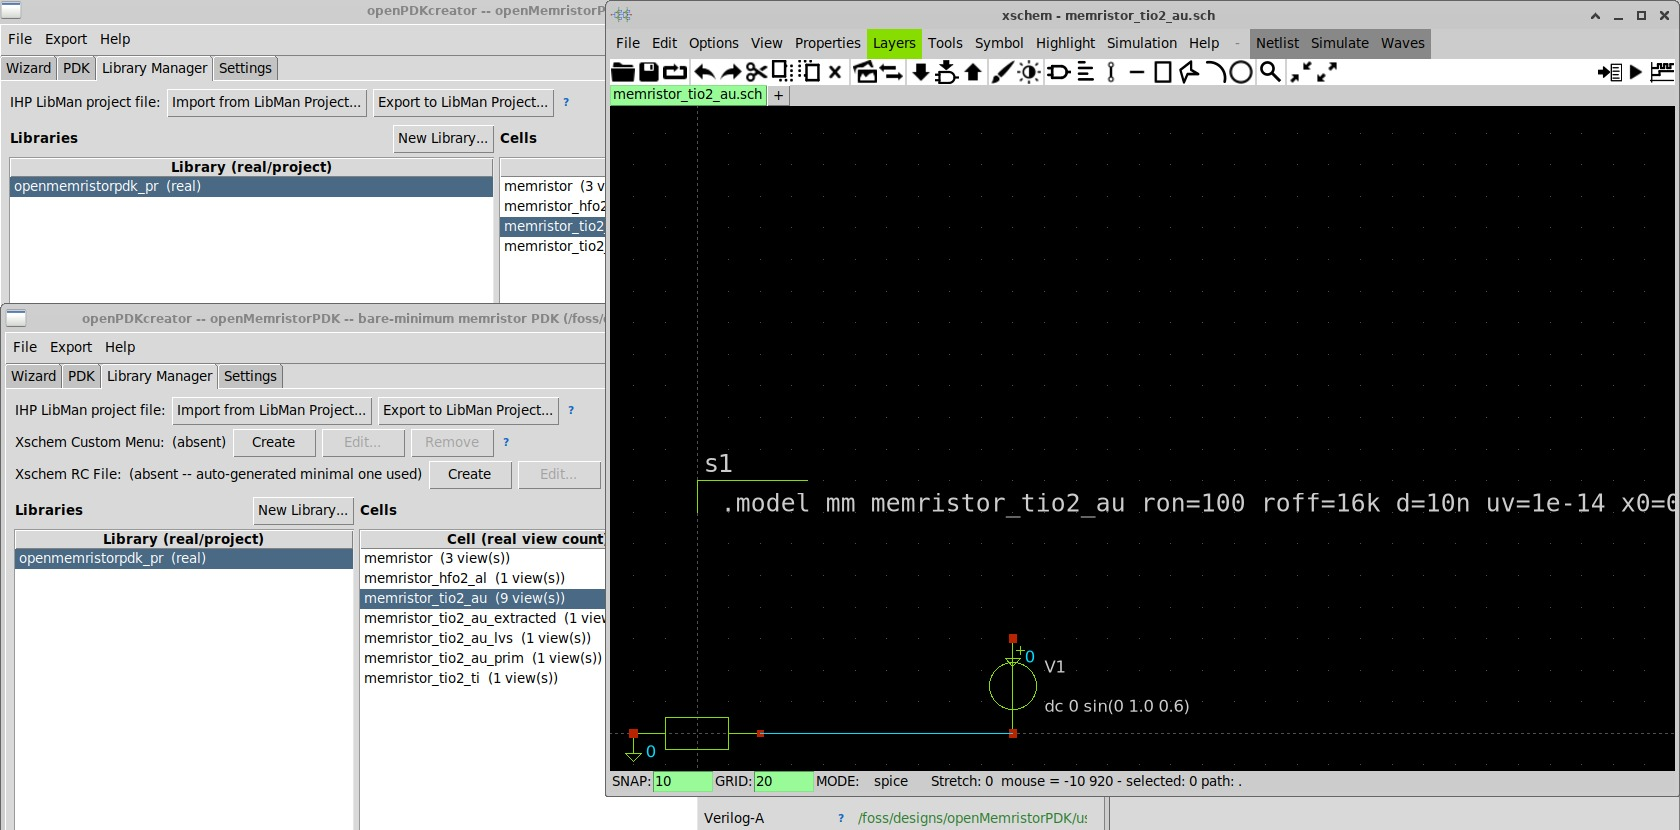
\includegraphics[width=0.55\textwidth]{figures/xschem_memristor_schematic.jpg}
\end{center}
\footnotesize
Memristor + \texttt{vsource} (xschem's own bundled device) + 2 real
grounds, wired. First real netlist attempt silently \emph{dropped}
the memristor instance entirely: the symbol's own \texttt{K
\{type=subcircuit\}} carried no real \texttt{format=} string. Fixed,
then a second real bug: \texttt{type=n name=1} emitted \texttt{X1}
(a real SPICE subcircuit-call prefix) instead of \texttt{n1} --
ngspice refused it (\texttt{unknown subckt: x1 ...}). The real fix:
the instance's own \texttt{name=} must carry its device-prefix letter
directly (\texttt{name=n1}), the same real convention xschem's own
\texttt{vsource.sym} uses (\texttt{name=V1}) -- found only by
actually running the generated netlist through real ngspice and
reading the real error.
\end{frame}

% ---------------------------------------------------------------
\begin{frame}[fragile]{The real, schematic-derived netlist}
\begin{cli}
xschem -n -s -q libraries/openmemristorpdk_pr/memristor_tio2_au.sch
\end{cli}
\begin{va}
n1 0 net1 mm
V1 0 net1 dc 0 sin(0 1.0 0.6)
.model mm memristor_tio2_au ron=100 roff=16k d=10n uv=1e-14 x0=0.3
\end{va}
Run through real ngspice/OSDI: resistance window
9343--16000\,$\Omega$ -- byte-for-byte the same real result as the
independently, directly hand-authored testbench earlier in this deck.
The real schematic and the real hand-written netlist agree exactly.
\end{frame}

% ---------------------------------------------------------------
\begin{frame}{What's real here -- and what's still a gap}
\begin{columns}
\column{0.5\textwidth}
\textbf{Real}
\begin{itemize}
  \item Independent project, own git history
  \item 6-layer, 2-material, 3-metal stack
  \item 2 real planes, 6 real Magic types
  \item 4 real DRC rules, real generated Ruby
  \item 4 real LEF macros, real port geometry
  \item 2 genuinely different Verilog-A models, 3 variants
  \item Real \texttt{openvaf} compiles, real \texttt{ngspice}
        transients for every variant
  \item Real TT/FF/SS corners, editable in-GUI
  \item Real xschem symbol + schematic, real launcher, real
        schematic-derived netlist matching the hand-written one
\end{itemize}
\column{0.5\textwidth}
\textbf{Known gaps (same honesty this
tool applies everywhere else)}
\begin{itemize}
  \item Only the Au/TiO$_2$/Au variant got a full schematic + real
        launcher round trip -- the other two variants' own
        simulations still use a directly hand-written testbench
        (see the earlier slides), not their own schematic
  \item Xschem symbol pin placement fought this session's own
        mouse-precision limits inside the tool's Tkinter canvas (a
        near-zero-size default pin target) -- finished via a small,
        direct, real-syntax text edit on the exported file instead
  \item Corner values are illustrative ($\pm$20\%), not calibrated
        against any real fabricated device
  \item No GDS/layout creation (same known limit as the IHP-based
        project)
\end{itemize}
\end{columns}
\end{frame}

% ---------------------------------------------------------------
\begin{frame}[fragile]{Where everything lives}
\begin{cli}
openMemristorPDK/
  data/openmemristorpdk/               # the live, editable PDK tree
  export/openmemristorpdk/             # real, open_pdks-format output
  libraries/openmemristorpdk_pr/
    memristor_tio2_au.sch              # real xschem schematic
  user_models/veriloga/
    memristor_tio2_au.va  memristor_tio2_ti.va  memristor_hfo2_al.va
  docs/simulation/
    memristor_tio2_au/  memristor_tio2_ti/  memristor_hfo2_al/
    memristor_tio2_au_corners/         # TT/FF/SS sweep
  saves/openmemristorpdk.yaml          # Magic Types/DRC/LEF/corners
\end{cli}
\end{frame}

\begin{frame}
\centering\Large Thanks!
\end{frame}

\end{document}
